\documentclass[aps,prl,reprint,groupedaddress]{revtex4-1}


\begin{document}

% Use the \preprint command to place your local institutional report
% number in the upper righthand corner of the title page in preprint mode.
% Multiple \preprint commands are allowed.
% Use the 'preprintnumbers' class option to override journal defaults
% to display numbers if necessary
\preprint{Demo Paper}

%Title of paper
\title{Demonstration of Scale Invariance at the Critical Point}

\author{Douglas J. Ashton}
\email[]{douglas.j.ashton@gmail.com}
\homepage[]{www.dougashton.net}
%\thanks{}
%\altaffiliation{}
\affiliation{Mango Solutions}


\date{\today}

\begin{abstract}
Critical point phenomena, such as scale invariance, and universality, can be difficult concepts to learn. Partly because it is difficult to visualise. The two dimensional Ising model is a very useful model to illustrate some of these behaviours due to its simplicity. This paper presents large scale, real space simulations of $ \tilde 10^10 $ lattice sites using a slightly modified Wolff algorithm. The configurations generated give a tangible demonstration of scale invariance.
\end{abstract}

% insert suggested PACS numbers in braces on next line
\pacs{1234}
% insert suggested keywords - APS authors don't need to do this
%\keywords{}

%\maketitle must follow title, authors, abstract, \pacs, and \keywords
\maketitle

% body of paper here - Use proper section commands
% References should be done using the \cite, \ref, and \label commands
\section{Introduction}{\label{sec-intro}}
% Put \label in argument of \section for cross-referencing
%\section{\label{}}
%\subsection{Introduction}

Most phase transitions are due to a competition between energy and entropy. On the one hand attractive forces want to pull particles together, and on the other entropy drives the particles to explore more configurations. This balance between energy and entropy is bourne out in the free energy, which may look like the following.

\begin{equation}
F = E - S k_B T
\end{equation}
where $E$ is the internal energy, $S$ the entropy, and $k_B T$ the temperature. High temperature favours entropy, low temperature favours energy.

A first order phase transition occurs when there is a discontinuity in the free energy with respsect to the order parameter. In a liquid-gas transition the order parameter is density. At the point of the discontinuity two very different phases, a high density liquid and a low density gas, have the same free energy and they can co-exist on either side of a phase boundary.

If we heat things up the boundary between the two begins to weaken and fluctuations between the phases grow stronger and stronger. At the critical point the fluctuations diverge. This is also known as a continuous phase, or second order, transition because there is no jump in free energy between the phases.

%% Maybe drop everything above and start below?

The behaviour of a material around its critical point is one of the strangest, and most beautiful results in statistical physics. The divergence in fluctuations creates a scale invariance with no length scale taking priority. This means that the details of what the liquid, or magnet, or other material, are made from becomes less important. The physics is instead driven by much simpler things such as dimensionality and symmtery. Thanks to this universality the critical point is one area where a simple model can produce exact results.

The theory of critical phenomena becomes quickly quite abstract making it difficult for students to gain a good intuition for the basic physical effect. In this paper we aim to demonstrate important consequences of scale invariance using a massive scale, real space simulation of the Ising model at its critical point. For this we use a modified version of the Wolff algorithm, designed to minimise the use of memory.

The paper is organised as follows: In the next section we present the model and simulation method and in the final section we show some key results.

\begin{figure}
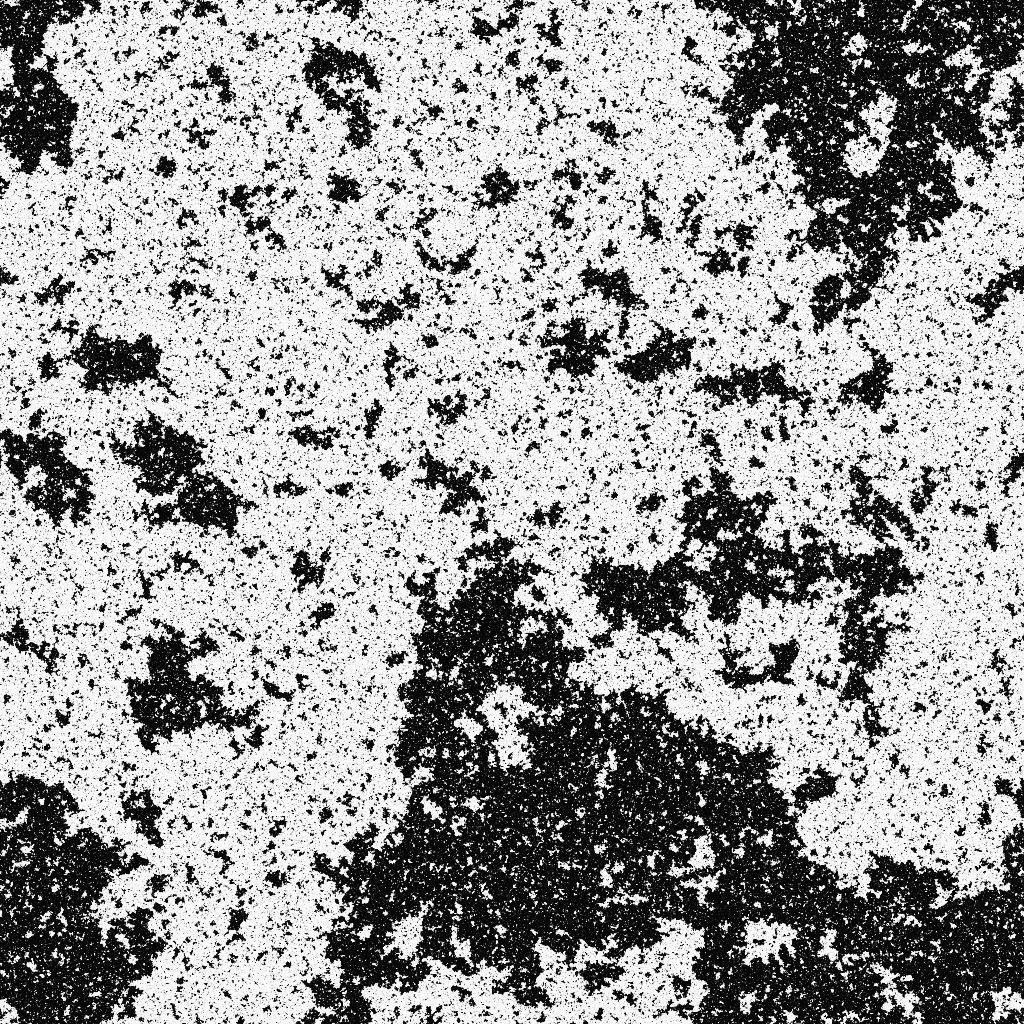
\includegraphics[width=\columnwidth]{data/swolff0000.png}
\caption{\label{fig-config} what}
\end{figure}

\section{Method\label{sec-method}}

\subsection{Ising Model}

The simplest model for system with attraction and randomness is the Ising model. The spin $\frac{1}{2}$ Ising model has spins arranged on a lattice able to point up ($\sigma = 1$), or down ($\sigma = -1$. In Fig. \ref{fig-config} these are shown with black or white pixels. The energy prefers spins to line up:

\begin{equation}
E = -J \sum_{i, j} \sigma_i \sigma_j
\end{equation}
where the sum is over all neighbouring pairs.

The two dimensional Ising model is the classic model to demonstrate critical phenomena. While it has been solved analytically in zero field CITE it is also useful for testing theories such as the renormalisation group CITE and demonstrating behaviour such as scale invariance CITE.

\subsection{Simulation Method}

Blah blah Wolff. 


\section{Results\label{sec-results}}

Results

\begin{figure}
\includegraphics[width=\columnwidth]{fig-density}
\caption{\label{fig-density} what}
\end{figure}

\begin{figure}
\includegraphics[width=\columnwidth]{fig-clusters}
\caption{\label{fig-clusters} what}
\end{figure}


% If in two-column mode, this environment will change to single-column
% format so that long equations can be displayed. Use
% sparingly.
%\begin{widetext}
% put long equation here
%\end{widetext}

% figures should be put into the text as floats.
% Use the graphics or graphicx packages (distributed with LaTeX2e)
% and the \includegraphics macro defined in those packages.
% See the LaTeX Graphics Companion by Michel Goosens, Sebastian Rahtz,
% and Frank Mittelbach for instance.
%
% Here is an example of the general form of a figure:
% Fill in the caption in the braces of the \caption{} command. Put the label
% that you will use with \ref{} command in the braces of the \label{} command.
% Use the figure* environment if the figure should span across the
% entire page. There is no need to do explicit centering.

% \begin{figure}
% \includegraphics{}%
% \caption{\label{}}
% \end{figure}

% Surround figure environment with turnpage environment for landscape
% figure
% \begin{turnpage}
% \begin{figure}
% \includegraphics{}%
% \caption{\label{}}
% \end{figure}
% \end{turnpage}

% tables should appear as floats within the text
%
% Here is an example of the general form of a table:
% Fill in the caption in the braces of the \caption{} command. Put the label
% that you will use with \ref{} command in the braces of the \label{} command.
% Insert the column specifiers (l, r, c, d, etc.) in the empty braces of the
% \begin{tabular}{} command.
% The ruledtabular enviroment adds doubled rules to table and sets a
% reasonable default table settings.
% Use the table* environment to get a full-width table in two-column
% Add \usepackage{longtable} and the longtable (or longtable*}
% environment for nicely formatted long tables. Or use the the [H]
% placement option to break a long table (with less control than 
% in longtable).
% \begin{table}%[H] add [H] placement to break table across pages
% \caption{\label{}}
% \begin{ruledtabular}
% \begin{tabular}{}
% Lines of table here ending with \\
% \end{tabular}
% \end{ruledtabular}
% \end{table}

% Surround table environment with turnpage environment for landscape
% table
% \begin{turnpage}
% \begin{table}
% \caption{\label{}}
% \begin{ruledtabular}
% \begin{tabular}{}
% \end{tabular}
% \end{ruledtabular}
% \end{table}
% \end{turnpage}

% Specify following sections are appendices. Use \appendix* if there
% only one appendix.
%\appendix
%\section{}

% If you have acknowledgments, this puts in the proper section head.
%\begin{acknowledgments}
% put your acknowledgments here.
%\end{acknowledgments}

% Create the reference section using BibTeX:
%\bibliography{basename of .bib file}

\end{document}
%
% ****** End of file apstemplate.tex ******

